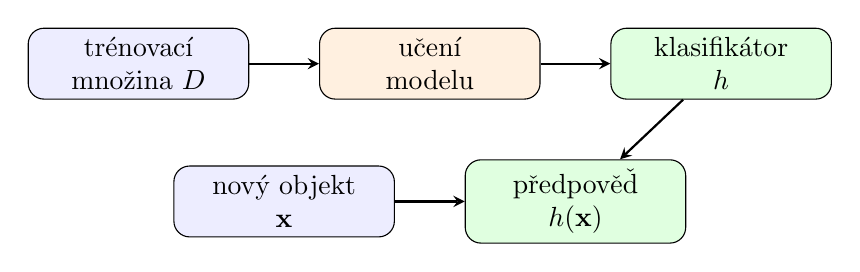
\begin{tikzpicture}[
    >=stealth,
    box/.style={
        draw,
        rounded corners=2mm,
        minimum width=28mm,
        minimum height=9mm,
        align=center
    },
    arr/.style={->, thick}
]
    \node[box, fill=blue!7] (data) at (0,0)
        {trénovací\\množina \(D\)};
    \node[box, fill=orange!12] (learn) at (3.7,0)
        {učení\\modelu};
    \node[box, fill=green!12] (model) at (7.4,0)
        {klasifikátor\\\(h\)};

    \node[box, fill=blue!7] (new) at (1.85,-1.75)
        {nový objekt\\\(\mathbf{x}\)};
    \node[box, fill=green!12] (out) at (5.55,-1.75)
        {předpověď\\\(h(\mathbf{x})\)};

    \draw[arr] (data) -- (learn);
    \draw[arr] (learn) -- (model);
    \draw[arr] (new) -- (out);
    \draw[arr] (model) -- (out);
\end{tikzpicture}
